

\begin{frame}{Decentral Control in Robot Teams}

\vspace{1em}
\justifying

We developed a {\bf decentral scheduling algorithm} that allows multiple robots 
to coordinate their behavior to achieve a common goal in a challenging, dynamic 
environment where communication might be intermittent and the number of robots 
might change without prior notice~\cite{Ziegler2004,Dahm2005a}. 
\vspace{1.5em}

\twocol{0.5}{
Characteristics of our approach:
\begin{itemize}
	\item synchronization free
	\item low-bandwidth broadcast communication
	\item graceful degradation in case of
	\begin{itemize}
		\item communication outages
		\item loss of team members
	\end{itemize}
	\item continuous replanning
\end{itemize}
}{0.41}{
\vspace{-2.5em}
\begin{figure}
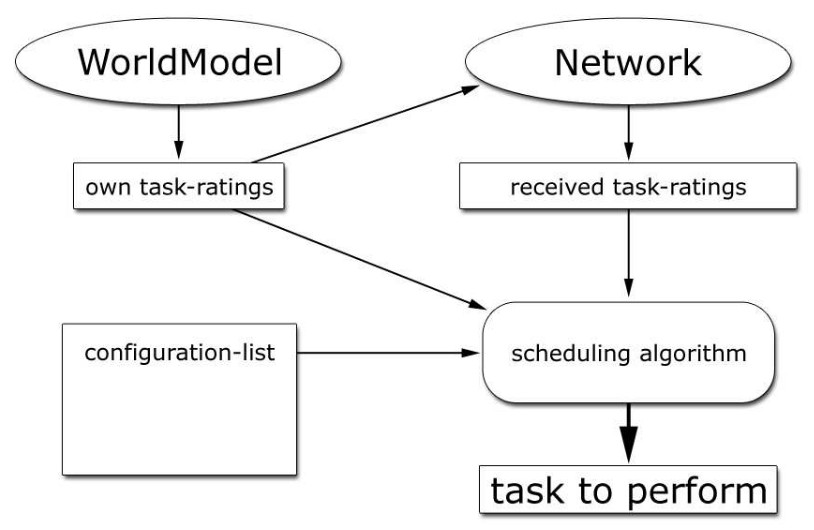
\includegraphics[width=0.9\linewidth]{decentral_control_in_robot_teams/schematic.jpg}

\vspace{-1em}
\caption{\scriptsize Schematic of the proposed scheduler (from~\cite{Ziegler2004}).}
\end{figure}
}
\vspace{1.25em}
The scheduling algorithm was successfully used during the RoboCup 2004 
competition winning the Standard Platform League Open Challenge~\cite{Dahm2004}.\vid{publications/2004-02/robocup04-gt_open_challenge.mp4}

\begin{center}
\rule{2cm}{0.4pt}\\[0.5em]
\end{center}

\fc{Ziegler2004}{publications/2004-01/2004-01}\\[1em]
\fc{Dahm2005a}{publications/2005-01/2005-01}

\end{frame}
